%%%%%%%%%%%%%%%%%%%%%%%%%%%%%%%%%%%%%%%%%%%%%%%%%%%%%%%%
% Este é um documento que servirá de modelo para
% os relatórios feitos na disciplina Circuitos Digitais
% 2016-2
%%%%%%%%%%%%%%%%%%%%%%%%%%%%%%%%%%%%%%%%%%%%%%%%%%%%%%%%%

\documentclass[12pt]{article}

\usepackage{sbc-template}
\usepackage[brazil,american]{babel}
\usepackage[utf8]{inputenc}

\usepackage{graphicx}
\usepackage{url}
\usepackage{float}
\usepackage{listings}
\usepackage{color}
\usepackage{todonotes}
\usepackage{algorithmic}
\usepackage{algorithm}
\usepackage{hyperref}
\usepackage{amsmath}
     
\sloppy

\title{Experimento 0\\ 
Conversores A/D e D/A }

\author{Isaac Lopes, 12/0120801\\
        Lucas Mafra Chagas, 12/0126443 \\
        Marcelo Giordano Martins Costa de Oliveira,  12/0037301
}


\address{Dep. Ciência da Computação -- Universidade de Brasília (UnB)\\
  CiC 116351 - Circuitos Digitais - Turma C
  \email{\{giordano.marcelo, chagas.lucas.mafra, isaaclopinho\}@gmail.com}
}

\begin{document} 

\maketitle

 \begin{abstract}
   This essay has the intention to show the results obtained by the students at the first contact with protoboard and digital amplifiers, showing, bulding and testing analog and digital converters circuits.
 \end{abstract}
     
 \begin{resumo} 
  Esse relatório tem o intuito de mostrar os resultados obtidos pelos alunos ao ter o primeiro contato com o protoboard e amplificadores digitais, apresentando, construindo e testando circuitos conversores de sinais análogicos e digitais.
 \end{resumo}


\section{1. Objetivos}
\label{sec:Objetivos}

Fornecer ao aluno um contato inicial com o protoboard e amplificadores operacionais.
Apresentar, construir e testar circuitos conversores de sinais analógicos e digitais.

\section{2. Materiais} 
\label{sec:Materiais}

\begin{itemize}
    
    \item \textit{protoboard}
    
    \item Fios
    
    \item Multímetro
    
    \item Resistores
    
    \item Ampop TL074
    
\end{itemize}


\section{3. Introdução}
\label{sec:Introducao}

No experimento de conversores D/A e A/D, será trabalhado a montagem de um circuito do Conversor Digital-Analógico com resistores ponderados, analisando a entrada de 3 bits e 4 bits. Além disso, será feito uma análise teórica do circuito do conversor Analógico-Digital tipo Flash.

\section{4. Procedimentos}
\label{sec:Procedimentos}

\begin{enumerate} 
	\item Montar o circuito do Conversor Digital-Analógico com resistores ponderados, mostrado na figura 1, fotografe o circuito final e preencher a tabela 1 com auxílio do multímetro. Após obter a tabela deve-se plotar o gráfico (código binário x Vout) e determinar o valor de tensão do fundo de escala e a resolução do conversor.

\begin{figure}[H]
\centering
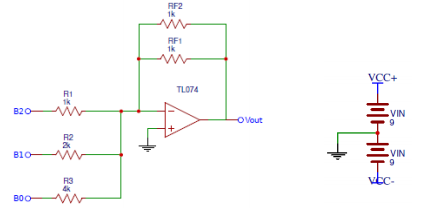
\includegraphics[width=.5\textwidth]{grafico3bitex.png}
\caption{ Circuito do conversor D/A de 3 bits.}
\label{fig:3bitex}
\end{figure}


	\item Acrescentar mais um bit de entrada no conversor D/A do paso anterior e refazer as medidas da tabela para o conversor de 4 bits. Após isso, determinar a tensão de fundo de escala e a resolução e plotar o gráfico (código binário x Vout), do conversor montado. 

	\item Fazer uma análise teórica do item 2.3 do experimento.
 
\end{enumerate}

\subsection{4.1 Conversor Analógico-Digital de 3 bits}
\label{sec:CAD3}


\begin{table}[H]
    \centering
    \caption{Valores de tensão Vout com 3 bits.}
    \begin{tabular}{|c|c|c|c|}
    \cline{1-4}
    \multicolumn{1}{|c|}{B2} & \multicolumn{1}{|c|}{B1} & \multicolumn{1}{c|}{B0} & \multicolumn{1}{|c|}{Vout} \\
    \hline
    0 & 0 & 0 & 0 \\
    0 & 0 & 1 & -0.71 \\
    0 & 1 & 0 & -1.44 \\
    0 & 1 & 1 & -2.15  \\
    1 & 0 & 0 & -2.86  \\
    1 & 0 & 1 & -3.57  \\
    1 & 1 & 0 & -4.28  \\
    1 & 1 & 1 & -4.91  \\
    \hline
    \end{tabular}
    \label{tab:resultado3bit}
\end{table}

Os valores acima correspondem os valores de saída do AmpOp correspondentes a cada combinação de 3 bits de entrada.

\begin{figure}[H]
\centering
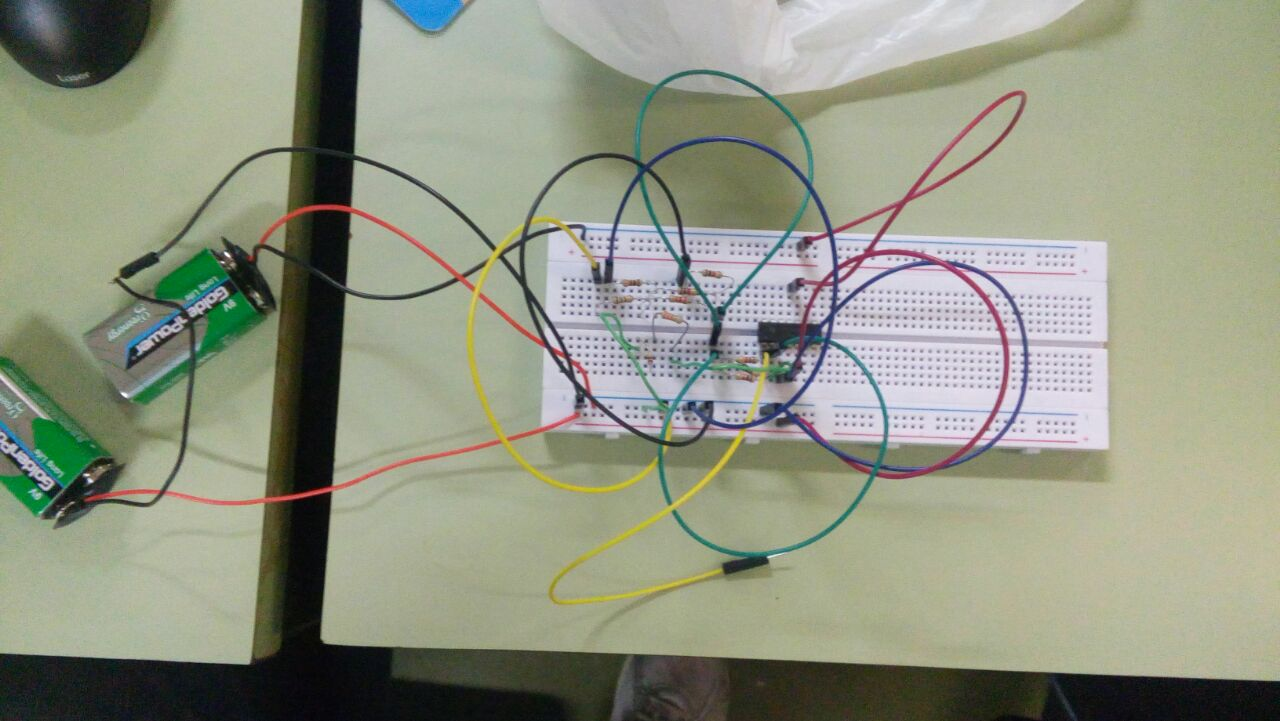
\includegraphics[width=.5\textwidth]{circuito.jpeg}
\caption{Circuito montado.}
\label{fig:circuito1}
\end{figure}


\begin{figure}[H]
\centering
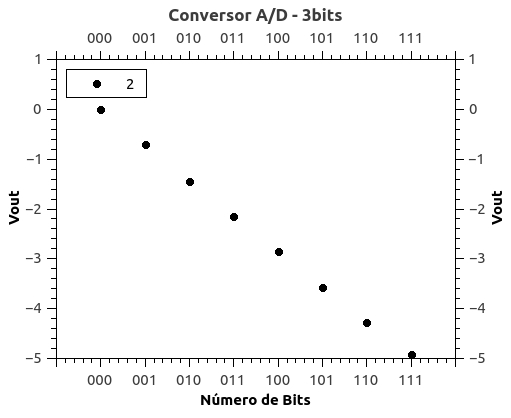
\includegraphics[width=.5\textwidth]{grafico3bitdot.jpeg}
\caption{Representação gráfica com pontos.}
\label{fig:3bitdot}
\end{figure}

\begin{figure}[H]
\centering
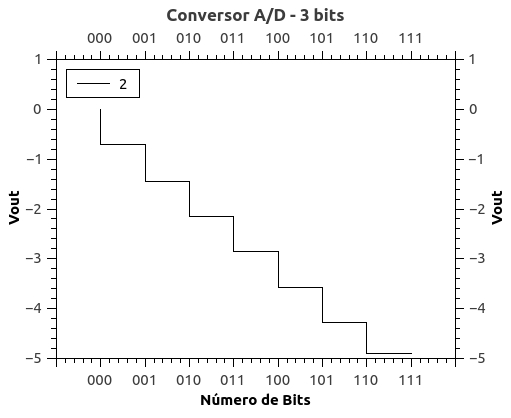
\includegraphics[width=.5\textwidth]{grafico3bit.jpeg}
\caption{Representação gráfica escada.}
\label{fig:3bit}
\end{figure}

Temos que o valor de \textit{Fundo de Escala} corresponde a \textbf{-4.91 V}. Já o valor da \textit{Resolução}, que é obtida na fórmula $R = \frac{Afs}{2^N-1}$ é igual a \textbf{0.7014 V}. Afs representa o valor da amplitude de fundo de escala e N o valor de bits.


\subsection{4.2 Conversor Analógico-Digital de 4 bits}
\label{sec:CAD4}


\begin{table}[H]
    \centering
    \caption{Valores de tensão Vout com 4 bits.}
    \begin{tabular}{|c|c|c|c|c|}
    \cline{1-5}
    \multicolumn{1}{|c|}{B3} & \multicolumn{1}{|c|}{B2} & \multicolumn{1}{|c|}{B1} & \multicolumn{1}{|c|}{B0} & \multicolumn{1}{|c|}{Vout} \\
    \hline
    0 & 0 & 0 & 0 & 0 \\
    0 & 0 & 0 & 1 & -0.36 \\
    0 & 0 & 1 & 0 & -0.72 \\
    0 & 0 & 1 & 1 & -1.08  \\
    0 & 1 & 0 & 0 & -1.46  \\
    0 & 1 & 0 & 1 & -1.81  \\
    0 & 1 & 1 & 0 & -2.17  \\
    0 & 1 & 1 & 1 & -2.52  \\
    1 & 0 & 0 & 0 & -2.89 \\
    1 & 0 & 0 & 1 & -3.24 \\
    1 & 0 & 1 & 0 & -3.59 \\
    1 & 0 & 1 & 1 & -3.94  \\
    1 & 1 & 0 & 0 & -4.30  \\
    1 & 1 & 0 & 1 & -4.65  \\
    1 & 1 & 1 & 0 & -4.99  \\
    1 & 1 & 1 & 1 & -5.33  \\
    \hline
    \end{tabular}
    \label{tab:resultado4bit}
\end{table}

Os valores acima correspondem os valores de saída do AmpOp correspondentes a cada combinação de 4 bits de entrada.

\begin{figure}[H]
\centering
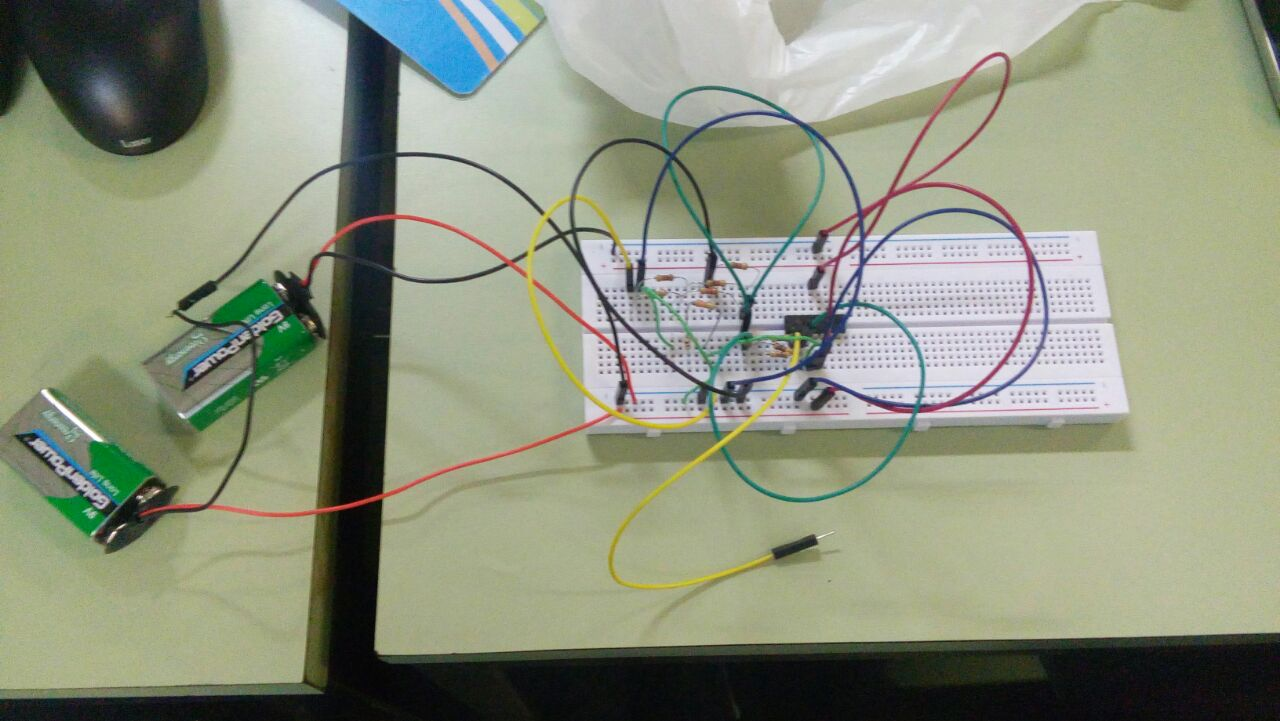
\includegraphics[width=.5\textwidth]{circuito2.jpeg}
\caption{Circuito montado.}
\label{fig:circuito2}
\end{figure}

\begin{figure}[H]
\centering
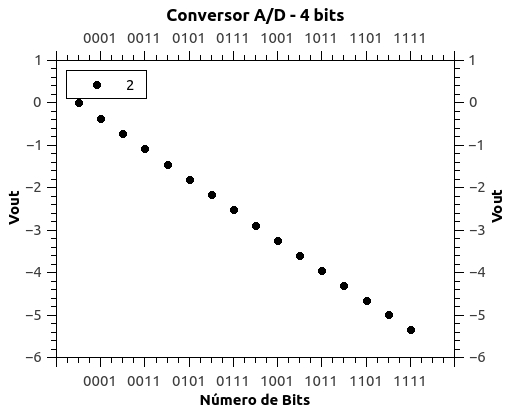
\includegraphics[width=.5\textwidth]{grafico4bitdot.jpeg}
\caption{Representação gráfica com pontos.}
\label{fig:4bitdot}
\end{figure}

\begin{figure}[H]
\centering
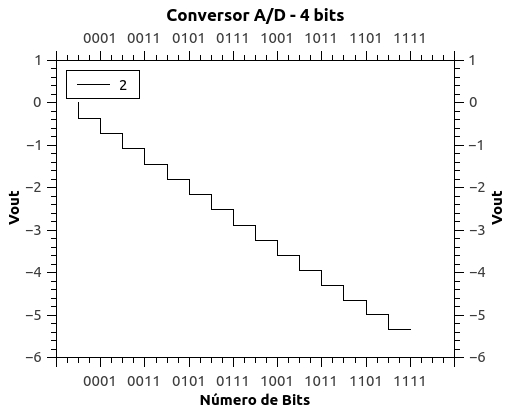
\includegraphics[width=.5\textwidth]{grafico4bit.jpeg}
\caption{Representação gráfica escada.}
\label{fig:4bit}
\end{figure}

Temos que o valor de \textit{Fundo de Escala} corresponde a \textbf{-5.33 V}. Já o valor da \textit{Resolução}, que é obtida na fórmula $R = \frac{Afs}{2^N-1}$ é igual a \textbf{0.3553 V}.  Afs representa o valor da amplitude de fundo de escala e N o valor de bits.


\subsection{4.3 Conversor Analógico-Digital Flash}
\label{sec:FLASH}


\begin{table}[H]
    \centering
    \caption{Valores de tensão Vout com 4 bits.}
    \begin{tabular}{|c|c|c|c|c|c|}
    \cline{1-6}
    \multicolumn{1}{|c|}{Vin min} & \multicolumn{1}{|c|}{Vin max} & \multicolumn{1}{|c|}{LED D1} & \multicolumn{1}{|c|}{LED D2} & \multicolumn{1}{|c|}{LED D3} & \multicolumn{1}{|c|}{LED D4} \\
    \hline
    0v & 1v & 0 & 0 & 0 & 0\\
    1v & 2v & 0 & 0 & 0 & 1\\
    2v & 3v & 0 & 0 & 1 & 1\\
    3v & 4v & 0 & 1 & 1 & 1\\
    4v & 5v & 1 & 1 & 1 & 1\\
    \hline
    \end{tabular}
    \label{tab:resultadoflash}
\end{table}

Nos dados anteriores, utilizamos voltagens teóricas para a realização da análise do experimento.

\begin{figure}[H]
\centering
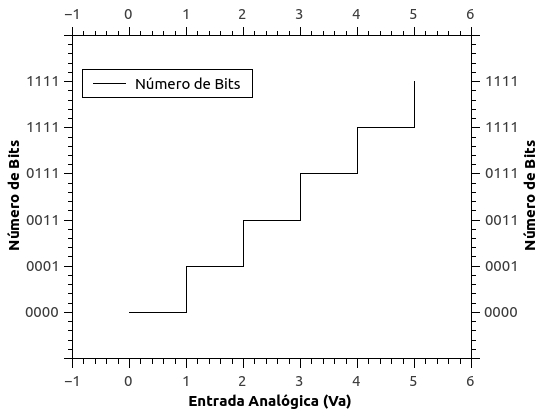
\includegraphics[width=.5\textwidth]{graficoconvadflash.jpeg}
\caption{Representação gráfica flash.}
\label{fig:graficoflash}
\end{figure}



\section{6. Conclusão}
\label{sec:Conclusao}

O experimento permitiu entender o funcionamento da protoboard, do multímetro digital e do amplificador operacional. Também, foi possível entender sobre sinais analógicos, digitais e como fazer a conversão destes a partir da montagem do circuito de conversor D/A, em caso de conversão do sinal digital para o sinal analógico, ou da montagem do circuito conversor A/D, caso contrário. Assim, o experimento foi bem sucedido.


\bibliographystyle{sbc}
\bibliography{relatorio}


\newpage 
% Colocar aqui apenas as respostas dos itens da Auto-Avaliação
\section*{7. Auto-Avaliação}

\begin{enumerate}
    \item C
    \item E
    \item C
    \item E
\end{enumerate}


\end{document}
